%
% $Id: ch01_overview
%
%   *******************************************************************
%   * SEE THE MAIN FILE "AllegThesis.tex" FOR MORE INFORMATION.       *
%   *******************************************************************

\chapter{Introduction}\label{ch:intro} % we can refer to chapter by the label

%   ************************************************************************
%   * In LaTeX, new paragraphs are begun by simply leaving a blank line in *
%   * the LaTeX file.                                                      *
%   *                                                                      *
%   * The \\ characters should NEVER be used to end a paragraph.           *
%   * They are used only for inserting line breaks in certain situations.  *
%   *                                                                      *
%   * "Widows" (ending paragraph lines at the top of a new page) and       *
%   * "orphans" (opening paragraph lines at the bottom of a page) should   *
%   * be eliminated; this sometimes requires re-writing some of the        *
%   * text to change the line lengths.                                     *
%   ************************************************************************

Sharing media with the public is becoming a more integral part of social interaction every day. Static images are just one of these many forms of media, and the number of daily uploads to image hosting websites is absolutely staggering. According to a recent survey by All Things Digital, as of May 2013, more than 500 million images are uploaded to image sharing websites each day, and this number is expected to double by the end of 2014 \cite{meek:500}. With figures this large, it immediately becomes apparent that multiple issues come with this trend of increased image sharing, namely, how much space does this number of images require, and is there a technology available to reduce this requirement? The simple answer is yes, there are tried and tested technologies that will reduce storage costs, but before looking into these technologies, it is important to understand what image hosting websites are and how they function.

\section{Image Hosting Services} \label{sec:imagehostingservices}
Image hosting services, or image sharing websites, are sites that allow users to upload images to the Internet and share them publicly with the link they are provided. These image sharing websites mostly operate in the same fashion, but recently a new breed has emerged. As seen in Figure \ref{imageshareprocess}, both submission processes are similar, but both have inherent advantages and disadvantages.

Looking at the first submission process variant at the top of Figure \ref{imageshareprocess}, a user would like to share an image with the public. The user can upload this image through the Internet from any Internet connected device, and the image will be stored on a publicly accessible server. From here, any number of people can access this shared image through an Internet-connected device indefinitely. Nearly all image hosting services operate on this model. Some of the more popular services include Flickr, Imgur, Photobucket, Shutterfly, and Instagram.

\begin{figure}[htbp]
\centering
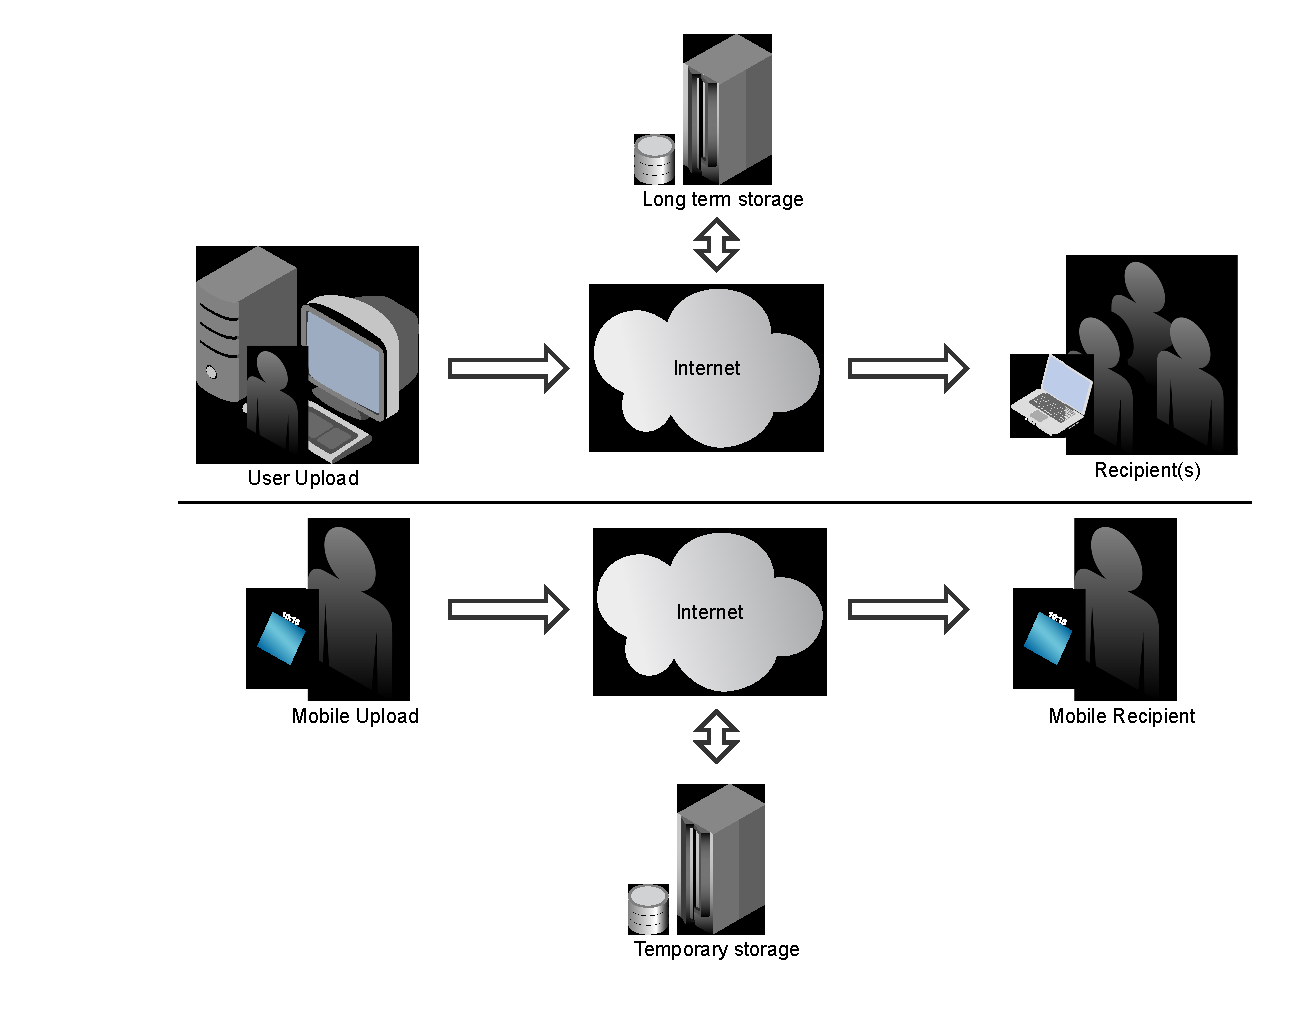
\includegraphics[width=4.5in]{imageshareprocess}
\caption{Various Image Hosting Service Structures}
\label{imageshareprocess}
\end{figure}

The second image submission variant shown at the bottom half of Figure \ref{imageshareprocess} is currently, as of December 2013, only used by one host called Snapchat. With this system, multiple differences are immediately apparent. First, this service model will accept images only from mobile users. It can also be seen in the diagram that when a user uploads an image through the Internet, it is no longer accessible long term from a server, but it is in fact only temporarily available for a specified recipient to receive. This service actually allows the uploader to set an expiration time anywhere from 1 second to 10 seconds \cite{snap:support}. After the recipient opens the image and this time period has expired, the image is deleted permanently from the server and no longer accessible to either party.

While both systems have their own inherent benefits, they also have drawbacks. Although they reach from the infrastructure needed to support the service all the way out to the end user, this research focuses only on the infrastructure function. In order to realize the application of the proposed research, it is important to understand why such a focused application is required. For the first image hosting variant in Figure \ref{imageshareprocess}, the long term storage of image files raises concern. By storing files for an extended period of time, it is a guarantee that duplicate data will make its way to the storage servers given enough time. Determining duplicates and preventing their addition can save not only a considerable amount of space as the amount of redundant data increases, but it can also save a large amount of money when discussing the cost per gigabyte of data storage which will be discussed in Section \ref{sec:motivation}. This research will not target the application of the temporary system seen at the bottom of the figure as the amount of stored data is comparatively minimal due to the rapid turnover of data being housed.

\section{Data Management Technologies} \label{sec:datadeduptech}
The image hosting services outlined in Section \ref{sec:imagehostingservices} utilize numerous technologies to help lessen the load of the files they must store. Although articles discussing the technologies these companies implement are nonexistent, after examining the services several different technologies became immediately apparent. The most prominent method of space reduction is the reduction in size of uploaded images. By reducing the quality of the image by a small percent, these websites are able to significantly reduce the amount of space needed to store the uploaded images. The next most common method of space reduction used is the expiration of uploads. After locating the earliest available images across the websites it was determined that the file expiration can possibly work in one of two ways. The implementation either functions as a countdown from the date of upload or in the other case the countdown begins after the last date the file was accessed. Each time the file is accessed, the timer will reset. Finally, some of these sites also limit the size of the uploaded files and the number of uploads per user. In order to remove these restrictions, many sites also offer paid services which help offset the cost of upkeep. 

\section{Motivation} \label{sec:motivation}
Summarizing the information presented thus far, image hosting websites clearly require complex infrastructures, not only to allow the sharing of files but to manage the large numbers of submissions. Although the numerous technologies used to lessen the space requirements of the submissions work well, it should be possible to further improve on the system by reducing the number of duplicate submissions. Remembering that more than 500 million images are uploaded to long-term image sharing websites each day, we have a baseline to calculate potential savings from. In addition, a study published by NTP Software found that nearly 20\% of stored data is duplicate \cite{ntps:staledata}. These numbers are staggering, especially when there is a possibility of reducing an additional 100 million images of required storage space.

To bring the possible savings into light a rough calculation based on the 2013 average of \$.05 per gigabyte and an assumed image size of 1MB will show that by removing the duplicates a significant amount of money could be saved. More specifically, approximately \$1.8 million can be saved annually at the current sharing levels. This number was calculated using the equation:
\begin{center}
$\frac{((Images_{Total}*\frac{\%Duplicate}{100})*365.25)*ImageSize_{Average}}{1024}*CostPerGB=TotalSavings$
\end{center}
Multiplying the total number of images uploaded each year by the percent duplicate we can find an approximation of how many duplicate images are stored annually. By multiplying this by the average image size we will know approximately how many megabytes of space this duplicate data will require to be stored. Finally, if we convert the cost per gigabyte to cost per megabyte to store the data and multiply that by the number of megabytes of data, the final cost per year to host this duplicate image data can be obtained. By allowing unregulated user submitted data, it quickly becomes apparent that data redundancy reduction can save a significant amount of storage space and money.

\section{Goals of the Project}\label{sec:goals}
This project develops and tests a system capable of efficiently identifying and reducing the number of duplicate image submissions on an image sharing website. In order to fulfill this goal, an image sharing website was developed which is capable of accepting images as uploads and providing a link to the user for public access of the image. To develop a functional website a set of requirements were met allowing it to perform several functions. The website was designed to accept an image file through an online submission form. At this point, it processes the image and matches it against a collection of images currently stored on the server. This process is completed using a series of algorithms and checks outlined in in Section \ref{ch:method}. The website was developed using PHP, the GD image library, and HTML5 to ensure minimal conflicts between scripts and languages. Using this site, the duplicate image detection tool was implemented using both original and existing code from other resources and tested thoroughly to assess the effectiveness of using this method of duplicate reduction.

\section{Thesis Outline}\label{sec:outline}
The remainder of this thesis will discuss the work in further detail in addition to existing information relating to the topic. Chapter \ref{ch:relatedwork} covers related works and existing research that has been completed on the topic of image matching and comparison. Chapter \ref{ch:method} covers the project details pertaining to the website and supporting infrastructure it will operate on. This includes a brief discussion of the hardware and configuration of the web server in addition to the website design and implementation of the duplicate image detection tool that will be integrated and tested. Chapter \ref{ch:reseval} discusses the collected results and the accompanying evaluation of the collected data. This evaluation includes the performance costs of implementing this system over a passive one, which only acts to prevent a specific file from ever being submitted to the server. The evaluation will also include the results of the image de-duplication and a determination of whether such a system is a feasible method of reducing storage requirements. An additional section outlining threats to validity will also be included in this chapter. Finally, Chapter \ref{ch:conclusion} summarizes the research and conclusions completed throughout this senior comprehensive project and include possible areas of future work.